\subsection{Expanded states and equivalent band} \label{app:expanded}

\begin{figure}[H]
  \centering
  \subfloat[$d{=}1\%$, exact matches]{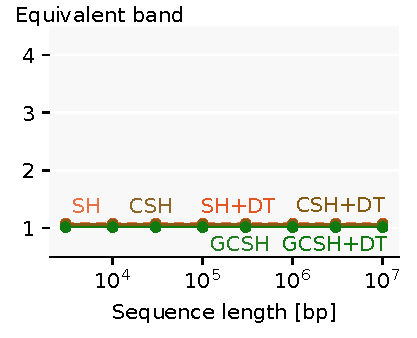
\includegraphics[scale=0.75]{plots/band_e0.01.labels.pdf}
  \label{fig:band1}}
  \hfill
  \subfloat[$d{=}4\%$, exact matches]{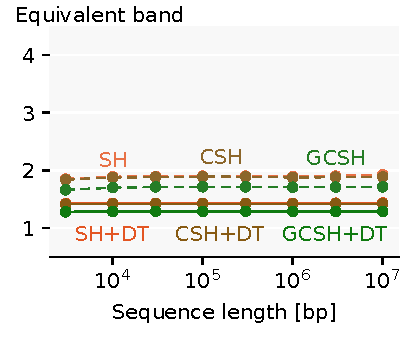
\includegraphics[scale=0.75]{plots/band_e0.05.labels.pdf}
  \label{fig:band5}}
  \hfill
  \subfloat[$d{=}8\%$, inexact matches]{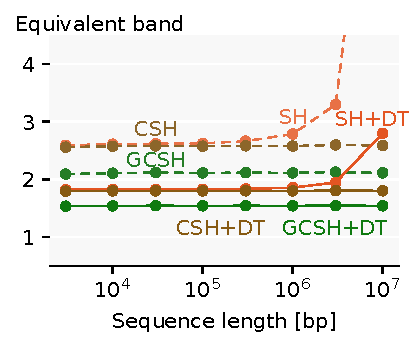
\includegraphics[scale=0.75]{plots/band_e0.10.labels.pdf}
  \label{fig:band10}}
  \hfill
  \subfloat[$d{=}12\%$, inexact matches]{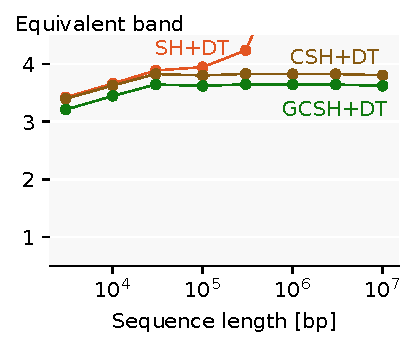
\includegraphics[scale=0.75]{plots/band_e0.15.labels.pdf}
  \label{fig:band15}}%
  \caption[Band scaling with sequence length on synthetic data]{\textbf{Equivalent band scaling with sequence length on synthetic data.}
    ($k{=}15$, $r{=}2$ for $d{\geq}8\%$). The equivalent band is the number of
    expanded states per bp for aligning synthetic sequences. Averages are over
    total $N{=}10^7\bp$. At $d{=}12\%$, the bands of non-DT methods are $\geq
    3\times$ wider.}
  \label{fig:band}
\end{figure}

The main benefit of an \A heuristic is a lower number of expanded states, which
translates to faster runtime. Instead of evaluating the runtime scaling with
length (\cref{fig:tools}), we can judge how well a heuristic
approximates the edit distance by directly measuring the \emph{equivalent band}
(\cref{fig:band}) of each alignment: the number of expanded states divided by
sequence length $n$, or equivalently, the number of expanded states per base pair.
The theoretical lower bound is an equivalent band of $1$, resulting from
expanding only the states on the main diagonal.

The equivalent band tends to be constant in $n$, indicating that the number of
expanded states is linear on the given domain. The equivalent band of \SH starts
to grow around $n\geq 10^6$ at divergence $d{=}8\%$, and around $n\geq 10^5$ at
$d{=}12\%$. Because of the chaining, \CSH and \GCH cope with spurious matches
and remain constant in equivalent band (i.e. linear expanded states with $n$).
The equivalent band for \GCH is slightly lower than \CSH due to better
accounting for indels. The DT variants expand fewer states by skipping
non-farthest reaching states.
